\section{Sviluppo dei contenuti}

\subsection{Esercizio unplugged}
Un operatore che si occupa di distribuire il contenuto di  un silos all'interno di svariati camion o carri ferroviari. Esistono condotte che collegano il silos ai vari punti di carico, che sono aperte e chiuse comandando delle valvole. 
Esistono più possibilità per comandare le valvole:
\begin{itemize}
\item O da linea di comando 
\item  Con GUI semplificata
\item Con GUI con schema di impianto

\end{itemize}
deve avere una consolle di comando in modo che possa capire velocemente in quale container mandare il materiale.
La consolle dal quale lo comanda come potrebbe essere strutturata, in che modo si può velocizzare e semplificare il lavoro dell'operatore?
Ecco due soluzioni proposte:
Soluzione  1 con CLI: istruzione del tipo: \texttt{switch valve N on/off} \newline
Soluzione 2 con GUI semplificata:
\begin{figure}
  \centering
  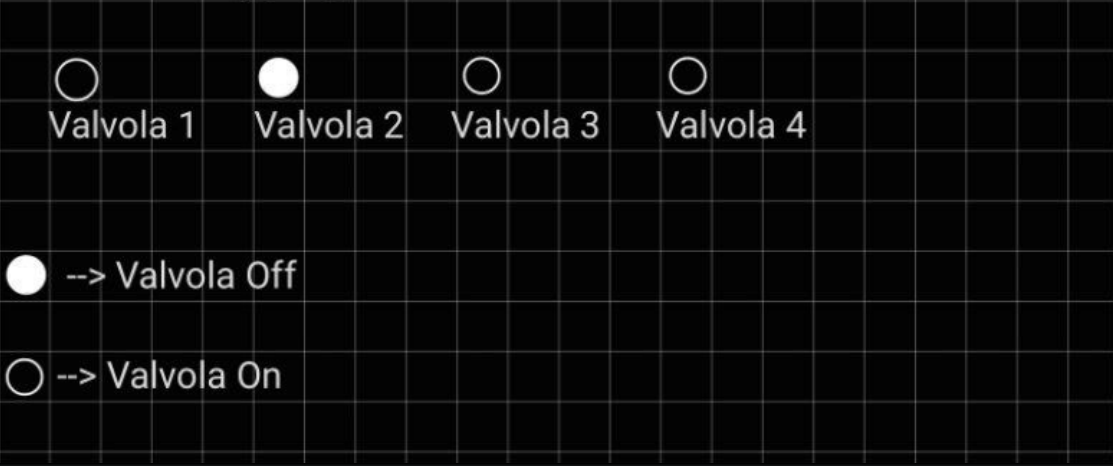
\includegraphics[width=0.5\textwidth]{img/gui_sempl.png}
  \caption{GUI semplificata}
\end{figure}


Soluzione 3: GUI con schema di impianto:
\begin{figure}
  \centering
  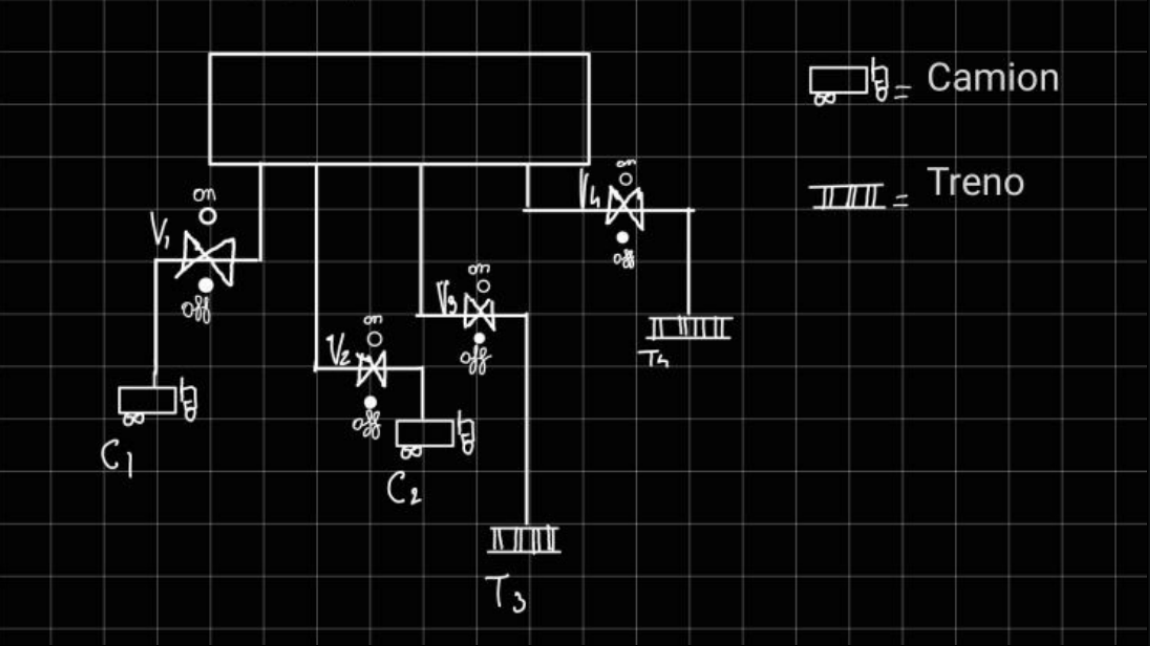
\includegraphics[width=0.5\textwidth]{img/gui_con_schema.png}
  \caption{GUI con schema di impianto}
\end{figure}


\subsection{Esercizi di programmazione cli-based}
Per iniziare a creare il programma, essendo GO un linguaggio che predilige la divisione in moduli, bisogna usare il comando seguente per creare il nuovo modulo nella cartella in cui si vuole creare il file con il codice sorgente \texttt{go mod init <nome\_modulo>}.\newline 
Questo creerà un file go.mod in cui viene specificato il nome del modulo (o package) e la versione di GO:
A questo punto si può creare il file ''.go'' dove scrivere il codice sorgente.
Questo codice deve svolgere i seguenti passaggi
\begin{itemize}
\item Chiedere all'utente il numero che vuole inserire
\item Leggere il numero
\item Calcolare il fattoriale del numero inserito
\item Stampare il risultato
\end{itemize}
Nb: il linguaggio permette di inserire in un'unica istruzione gli ultimi due passaggi

\begin{verbatim}
  
package main

import (
	"fmt"
)

func factorial(n int) int {
	if n == 0 {
		return 1
	} else {
		return n * factorial(n-1)
	}
}

func main() {
	var n int
	fmt.Println("Enter a number: ")
	fmt.Scan(&n)
	fmt.Printf("The factorial of %d is: %d ", n, factorial(n))
}
\end{verbatim}
\begin{quote}
In questo frammento di codice, troviamo due istruzioni caratteristiche del linguaggio, ovvero:
\end{quote}
\begin{itemize}
\item package main, serve identificare dove andrà la funzione \emph{main} che serve a dare un inizio al codice.
\item  import ''fmt'', questa parte serve a dire che librerie verranno importate nel codice, fmt è la libreria standard di Go che si occupa di fornire le funzioni per elaborare I/O la sua corrispondente in C è \emph{stdio}
\end{itemize}
\subsection{Esercizi di programmazione gui-based}
Analogamente alla parte precedente, creiamo una cartella un'altra cartella di lavoro per il medesimo programma ma con una GUI, e generiamo il modulo con il comando spiegato precedentemente. Essendo una GUI più complicata da costruire, il codice sorgente sarà nettamente più lungo, infatti non useremo una libreria standard ma una libreria esterna, che si può facilmente installare attraverso il comando:
\texttt{go get github.com/gotk3/gotk3/gtk} \newline

Questo comando ''preleva'' la libreria e creerà un file go.sum usato per tenere traccia delle librerie esterne usate nel codice sorgente e aggiungerà la libreria richiesta al file go.mod. 
A questo punto si può creare il codice sorgente che svolga  le seguenti fasi:
\begin{itemize}
\item Creare una prima finestra che poi andrà riempita con le varie parti
\item Creare una griglia e un' ''etichetta'' dove andremo a mettere un'istruzione per l'utente su cosa deve fare e un'etichetta dove verrà mostrato il risultato
\item Un ''entry'' dove l'utente inserirà i numeri (NB  verranno letti come una stringa, quindi verrà convertito con la funzione Atoi())
\item Un bottone per calcolare il fattoriale del numero inserito
\item Infine ''collegare'' il bottone alla funzione effettiva per ottenere il fattoriale
\end{itemize}
NB: La libreria esterna non ha una vera e propria gestione degli errori, per questo nel codice sorgente insieme ogni dichiarazione di una variabile per creare le varie parti della GUI viene dichiarata una variabile err e viene sempre controllato che sia nulla. infatti nel caso questa variabile abbia un valore non nullo vuol dire che qualcosa è andato storto nella creazione del componente.
\begin{verbatim}
  
  package main
  
  import (
    "fmt"
    "github.com/gotk3/gotk3/gtk"
    "log"
    "strconv"
  )
  
  func factorial(n int) int {
    if n == 0 {
      return 1
    } else {
      return n * factorial(n-1)
    }
  }
  
  func calculateFactorial(button *gtk.Button, entry *gtk.Entry, label *gtk.Label) {
    numStr, err := entry.GetText()
    if err != nil {
      log.Fatal("Error getting input:", err)
    }
  
    num, err := strconv.Atoi(numStr)
    if err != nil {
      log.Fatal("Error converting input to integer:", err)
    }
  
    result := factorial(num)
    label.SetText(fmt.Sprintf("The factorial of %d is: %d", num, result))
  }
  
  func main() {
    gtk.Init(nil)
  
    builder, err := gtk.BuilderNew()
    if err != nil {
      log.Fatal("Error initializing GTK builder:", err)
    }
  
    err = builder.AddFromFile("gui.glade")
    if err != nil {
      log.Fatal("Error loading UI file:", err)
    }
  
    obj, err := builder.GetObject("window1")
    if err != nil {
      log.Fatal("Error getting window object from UI file:", err)
    }
  
    window, ok := obj.(*gtk.Window)
    if !ok {
      log.Fatal("Error casting window object from UI file")
    }
  
    window.Connect("destroy", gtk.MainQuit)
  
    obj, err = builder.GetObject("button1")
    if err != nil {
      log.Fatal("Error getting button object from UI file:", err)
    }
  
    button, ok := obj.(*gtk.Button)
    if !ok {
      log.Fatal("Error casting button object from UI file")
    }
  
    obj, err = builder.GetObject("entry1")
    if err != nil {
      log.Fatal("Error getting entry object from UI file:", err)
    }
  
    entry, ok := obj.(*gtk.Entry)
    if !ok {
      log.Fatal("Error casting entry object from UI file")
    }
  
    obj, err = builder.GetObject("label1")
    if err != nil {
      log.Fatal("Error getting label object from UI file:", err)
    }
  
    label, ok := obj.(*gtk.Label)
    if !ok {
      log.Fatal("Error casting label object from UI file")
    }
  
    button.Connect("clicked", calculateFactorial, entry, label)
  
    window.ShowAll()
  
    gtk.Main()
  }
  \end{verbatim}
  